%% Extracted from D-figures.tex 2026-10-08 so it can sit in the
%% BODY, beside the text that discusses it, rather than in an
%% appendix. Exactly one definition: D-figures.tex no longer has
%% a copy.
\begin{figure}[t]
\centering
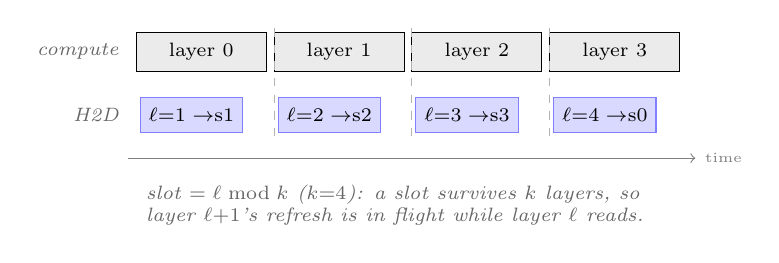
\begin{tikzpicture}[
  x=1cm, y=1cm, font=\scriptsize,
  cmp/.style={draw, fill=black!8, minimum height=5mm, inner sep=1pt},
  xfer/.style={draw, fill=blue!15, draw=blue!50, minimum height=4.5mm, inner sep=1pt},
  lbl/.style={font=\scriptsize\itshape, text=black!60},
]
\node[lbl, anchor=east] at (-0.1,0.2) {compute};
\foreach \i/\x in {0/0,1/1.75,2/3.5,3/5.25}
  \node[cmp, minimum width=1.65cm] at (\x+0.825,0.2) {layer $\i$};

\node[lbl, anchor=east] at (-0.1,-0.6) {H2D};
\foreach \i/\x/\s in {1/0/1,2/1.75/2,3/3.5/3,4/5.25/0}
  \node[xfer, minimum width=1.3cm] at (\x+0.70,-0.6) {$\ell{=}\i\rightarrow$s\s};

\foreach \x in {1.75,3.5,5.25} \draw[dashed, black!30] (\x,0.5) -- (\x,-0.95);
\draw[->, black!50] (-0.1,-1.15) -- (7.1,-1.15) node[right, font=\tiny] {time};

\node[lbl, anchor=west, align=left] at (0,-1.75)
  {slot $= \ell \bmod k$ ($k{=}4$): a slot survives $k$ layers, so\\
   layer $\ell{+}1$'s refresh is in flight while layer $\ell$ reads.};
\end{tikzpicture}
\caption{\textbf{Per-layer pipeline.} The refresh for layer $\ell{+}1$ is issued
while layer $\ell$ computes. $k$ slots give a transfer $k{-}1$ layers of slack
before its destination is reused, which is what allows it to be hidden;
$k{=}1$ would serialise transfer against compute. \S\ref{sec:eval:cost}
measures the fraction actually hidden.}
\label{fig:pipeline}
\end{figure}
